\chapter{Konzeptionierung des Educational Games}

\section{Mögliche Technologien zur Erstellung von TLT}

In Kapitel \ref{bisherigeTechnikTLT} kann nachgelesen werden, auf welchen Technologien TLT basiert. Für die Weiterentwicklung im Rahmen dieses Projektes wird auch mit neuen Techniken gearbeitet. Diese sollen hier kurz erläutert werden, bevor dann im Kapitel 5 detaillierter auf die Umsetzung eingegangen wird. 

Das Regelwerk, eine der drei Schichten, wird weiterhin in Java implementiert sein. Da diese Umsetzung einwandfrei funktioniert, ist es nicht sinnvoll, viel Zeit in eine neue Implementierung zu investieren. Bis auf kleine Veränderungen welche für bestimmte Lektionen nötig sind soll hier nichts verändert werden. 

Erweitert wird das "`Fundament"' von TLT um die nötigen AI-Algorithmen. Diese sollen ähnlich dem Prinzip von Modulen in das Projekt eingebunden werden. Als erste Wahl für eine Programmiersprache wurde Python gewählt. Wie viel während der Umsetzung wirklich in Python programmiert wird, muss sich erst noch zeigen. Diese ersten Überlegungen werden im späteren Kapitel \ref{umsetzungchapter} über die Umsetzung weitergedacht.

Als Datenhaltung wird im Hintergrund eine Datenbank aufgesetzt, die die wichtigsten Daten speichert. Das sind vor allem Bildschirmtexte, Parameter und Spielerinformationen. 

An die Oberfläche werden ebenfalls einige Anforderungen gestellt. Sie soll einfach zu bedienen und zu verstehen sein, da es hinderlich wäre, wenn der Anwender erst die UI verstehen muss. Die Implementation darf nicht zu zeitaufwändig sein. Angestrebt wird ein aus dem Web aufrufbares Interface, in dem dann mit einem Konto gearbeitet werden kann. Alternativ bietet sich auch eine Anwendung an, welche mit einer GameEngine realisiert wird.

\section{Welche AI-Technologien können mit TLT gelernt werden}
\label{lernbareTechnologien}

Zunächst kann mit TLT allgemeines Wissen im Bereich AI erworben werden. TLT gibt neben einem Überblick über verschiedene Einsatzgebiete auch grundlegende Definitionen und Erklärungen zu den verschiedenen Techniken und Ansätze im Bereich \textit{Machine Learning}. Ebenfalls bekommt der Spieler einen Einblick in die Funktionsweise und den Aufbau von (verschiedenen) Neuronalen Netzen. Für den geschichtsinteressierten Spieler gibt es die Möglichkeit etwas über die Vergangenheit der Neuronalen Netze zu lernen.

Hat der Spieler diese Grundlagen durchlaufen hat er die Möglichkeit in verschiedenen Lernbausteinen verschiedene Technologien kennen zu lernen. Aufgrund dem begrenzten Zeitrahmen dieser Studienarbeit wird zunächst nur ein Lernbaustein bearbeitet.

Dabei fiel die Wahl auf \textit{Deep Learning}. Dies hatte verschiedene Gründe. Zum einen bietet sich \textit{Deep Learning} aufgrund seiner \glqq einfachen\grqq{} Art sehr gut für einen geeigneten Einstieg an. Zum anderen stellt \textit{Deep Learning} auch den aktuellen Trend dar. Viele Firmen nutzen aktuell diese Technologie und es gibt eine Flut von Erklärungen und Bibliotheken. Mit TLT soll dem Spieler die Suche nach einem passenden Tutorial abgenommen werden.

Eine genaue Umsetzung der Lernmethodik für diese Themen kann in Kapitel \ref{lernmethodik_chapter} nachgelesen werden.


\section{Game Design}
\label{strukturlobby}

Game Design beschreibt das Gestalten des Spiels in seiner Logik und ist nicht zwingend auf die UI bezogen. In diesem Abschnitt soll für die verschiedenen zu erstellenden Bereiche beschrieben werden, wie dies realisiert werden könnte.

\subsection{Intro}
\label{lm_intro}

Das Intro von The Learning Triangle hat zwei grundlegende Aufgaben: Es soll eine Einführung in die Bedienung des Spiels geben, da dabei Dinge wie beispielsweise Navigation durch Menüs und Durchführen von Aktionen von Relevanz sind. Als weitere Aufgabe gilt es, die Grundlagen von TLT zu erklären und dem Spieler die Umgebung des Spiels vertraut zu machen.

Voraussetzung für das Intro ist die erstmalige Anmeldung eines Spielers. Dabei ist das Abschließen dieser Lektion verpflichtend, um weitere Lektionen spielen zu können. Das liegt am hier vermittelten Wissen, welches für nahezu alle späteren Bereiche relevant ist. Spielt ein Spieler das Spiel zum ersten Mal wird er automatisch in das Intro versetzt.

Zu Beginn ist nichts zu sehen, bevor dann nach kurzer Zeit eine Textbox mit Informationen eingeblendet wird. Die Textbox erklärt sich selbst und hilft dem Spieler, die ersten Interaktionen mit dem Spiel zu machen. Dazu zählt beispielsweise das Bestätigen von Anweisungen oder die Funktion bestimmter Tasten. Selbsterklärende Aktionen wie Scrollen durch Text werden dabei vorausgesetzt.  \newline  \newline

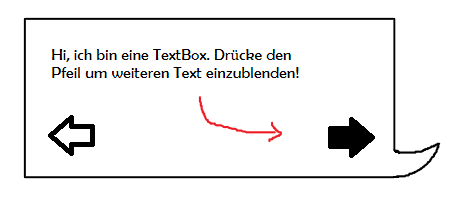
\includegraphics[scale=1.1]{bilder/Textbox.png}\\[5ex]

Nach der Einführung in die Bedienung wird nun das erste Mal eine leere Spielwelt von TLT eingeblendet. Dieser Schritt wird getan, da anhand der leeren Welt viel einfacher erklärt werden kann, welche Eigenschaften alle Welten teilen, als das eine Fülle von Text tun könnte. Generell soll unnötig viel Text immer vermieden werden, da die Motivation darunter leidet. Aussagekräftige, ergänzende Information werden trotzdem eingeblendet.

Direkt im Anschluss wird das Triangle in die Welt gesetzt, bevor es dann nach einer kurzen Erläuterung mit eigenständiger Bewegung beginnt. Auch hier soll mit zusätzlichen, kurzgehaltenen Texten erklärt werden, was dabei passiert und wieso es beispielsweise Energie kostet, Bewegung durchzuführen. Ebenfalls soll gezeigt werden, das Triangles sterben können.

Nun werden Felder eingeführt, welche verschiedene Einflüsse auf das Triangle ausüben. Die Funktion dieser soll dem Nutzer erklärt werden, in dem das Triangle demonstrativ auf die Felder bewegt wird und die Aktion direkt visuell einsehbar ist. Dabei wird dem Nutzer die Aufgabe gegeben, das Triangle zu steuern und für jeden Feldtyp zu testen, welche Konsequenz entsteht.

Nach der Erklärung der Felder wird die letzte wichtige Variable, das Sichtfeld des Triangles, erläutert. Hier ist ebenfalls eine Visualisierung eines Sichtfeldes um ein Triangle herum der beste Weg, um die Funktion und Auswirkung zu erklären. Dazu werden alle Felder, welche nicht im Sichtfeld liegen, ausgegraut. Anschließend soll der Nutzer das Triangle erneut selbst steuern können und muss mit einem Sichtfeld durch ein ihm unbekanntes Labyrinth aus Feldern zum Ziel kommen. Das verdeutlicht die Wichtigkeit des Sichtfeldes für weitere Aufgaben.

An diesem Punkt ist das Intro beendet und der Nutzer wird in das Hauptmenü versetzt. Wie genau dieses aufgebaut ist und welche wichtigen Elemente beachtet werden müssen, lässt sich in Kapitel \ref{strukturlobby} nachlesen.

\subsection{Die Lobby}

Nach dem in Abschnitt \ref{lm_intro} beschriebenen Intro gelangt der Spieler in die sogenannte Lobby. Diese ist der Mittelpunkt des Spiels und wird in folgendem Abschnitt genauer beschrieben. 

Die Lobby ist das Menü des Spiels, von dem aus der Spieler in die verschiedenen Lektionen gelangt, sowie die Referenzen einsehen und Hilfe bekommen kann. Abbildung \ref{BildLobby} zeigt den Aufbau der Lobby, welcher dem Spieler mit Hilfe der im Intro eingeführten Sprechblasen (dunkelgrün) erklärt wird. 

Dabei wird jedoch nicht einfach ein Menü integriert, über das der Benutzer seine Auswahl treffen kann. Es soll ein interaktiver Bildschirm sein, in dem die Möglichkeiten gestalterisch in die Thematik eingebunden sind. Dabei wird eine aus TLT bekannte Map aufgebaut, die der Benutzer erkunden kann. Von dort gelangt er in die verschiedenen Lektionen und gewöhnt sich sofort an die Umgebung eines Spiels. Das soll aber nicht ausschließen, dass auch ein Menü gebraucht wird, da nicht jeder Spaß an dieser Gestaltung hat. Außerdem hat es den Nachteil, dass Orientierung und mehr Zeit benötigt wird, um ein gewünschtes Ziel zu erreichen, ein Problem welches in einem Menü nicht existiert.

\begin{figure}[ht]
\centering
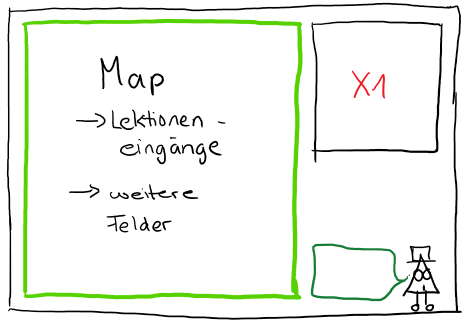
\includegraphics[scale=1.1]{bilder/Lobby.PNG}
\caption{Die Lobby}
\label{BildLobby}
\end{figure}

Der Bereich rechts oben, mit X1 betitelt, beinhaltet Platz für die Hilfe, die Referenzen und einen Shop, in dem der Spieler besondere Dinge für die im Spiel gewonnene Energie kaufen kann. Unterhalb befindet sich der Bereich, in dem eine Sprechblase immer dann abgebildet wird, wenn es etwas zu erklären gilt.

Der große Hellgrün markierte Bereich beinhaltet die Spielmap. Über diese Map gelangt der Spieler zum Beispiel in die verschiedenen Lektionen. Abbildung \ref{BildBeispielMap} zeigt, wie solch eine Map von der Art her aussehen könnte. Natürlich ist dies nur ein erster Entwurf, die reale Implementierung kann von diesem Bild abweichen. Grundlegend geht es aber darum, zu verstehen, wie die Map aufgebaut ist. Die Map ist aus folgenden Feldern aufgebaut:

\begin{center}
\label{tbl_mapFields}
\begin{tabular}{ |p{2cm} |p{3.1cm} | p{7.9cm}| c r r }
\hline
Zeichen & Feld & Bedeutung \\
\hline

\includegraphics[scale=1.1]{bilder/Wand.png} & Wände & Durch Wände kann der Spieler sein Dreieck nicht steuern. \\  
\hline
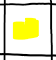
\includegraphics[scale=1.1]{bilder/Energie.png} & Energie & Energiefelder erhöhen das Energielevel des Spielers. \\
\hline
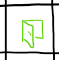
\includegraphics[scale=1.1]{bilder/Lektioneneingang.png} & Lektioneneingänge & Über die Lektioneneingänge kommt der Spieler in eine neue Lektion. \\ 
\hline
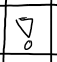
\includegraphics[scale=1.1]{bilder/Erklaerungen.png} & Erklärungen & Hier wird dem Spieler das Thema der Lektion aufbereitet erklärt. \\
\hline
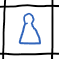
\includegraphics[scale=1.1]{bilder/Spiele.png} & Spiele & Hier finden sich die Spiele der Lektion zum nochmal spielen. \\
\hline
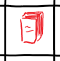
\includegraphics[scale=1.1]{bilder/referenzen.png} & Referenzen & Die passenden Referenzen zur Lektion. Durch überlaufen des Feldes wird der Bereich in der Bibliothek freigeschaltet. \\
\hline
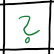
\includegraphics[scale=1.1]{bilder/Quiz.png} & Quiz & Die Möglichkeit sein Wissen über ein Quiz zu testen.\\
\hline
\end{tabular}
\end{center}

\newpage

\begin{center}
\begin{figure}[ht]
\centering
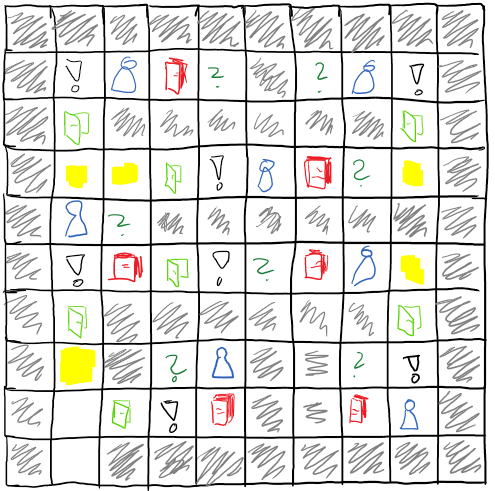
\includegraphics[scale=1.1]{bilder/BeispielMap.png}
\caption{Beispielhafte Map}
\label{BildBeispielMap}
\end{figure}
\end{center}

\newpage

Der Spieler kann mit Hilfe der Pfeiltasten seiner Tastatur das Dreieck über die Map bewegen. Befindet er sich auf einem Aktionsfeld (wie zum Beispiel einem Lektioneneingang oder dem Quiz Feld) kann der Spieler über \glqq Enter \grqq die jeweilige Aktion auslösen.

Allerdings ist zu Beginn des Spiels nicht die gesamte Map für den Spieler frei zugänglich. Je mehr Lektionen erfolgreich bestanden wurden, desto mehr ausgegraute Fläche der Map wird spielbar. Dies soll verhindern, dass der Spieler eine Lektion spielt, welche ein gewisses Vorwissen aus einem vorherigen Level benötigt. Gleichzeitig kann so auf geschickte Weise ein roter Faden durch die Lernstruktur eingebunden werden.


\subsection{Verwendete Elementen eines Educational Games}

Das Ziel des Spiels im Allgemeinen ist Wissen über AI auf eine Art und Weise zu vermitteln, welche Spaß macht. Das Ziel des Spielers ist es, am Ende in diesem Themengebiet alle nötigen Grundlagen zu beherrschen, sich mit den verschiedenen Richtungen auseinandergesetzt zu haben sowie durch nach-programmierte Codebeispiele in der Lage ist, die verschiedenen Technologien anzuwenden. 

Da es ein langer Weg bis dorthin ist und die Motivation sich etwas Neues anzueignen oftmals nicht sehr lange anhält, gibt es in dem Spiel ein Belohnungssystem, welches in leicht abgewandelter Form auf dem Energiesystem des namensgebenden Dreiecks basiert. Schließt der Spieler eine Lektion erfolgreich ab, so erhält er Energie. Ebenso wenn er zum Beispiel in einem Quiz eine Frage richtig beantwortet, oder eine Aufgabe in einer Lektion erfolgreich löst. Die gewonnene Energie kann in einem internen Shop zu Ausrüstung des Dreiecks ausgegeben werden. Das Sammeln von Energie soll dazu verhelfen, dass der Spieler Spaß hat und das Weiterspielen zum eigenen Wunsche wird, und nicht, weil der Spieler das Themengebiet lernen muss.

Ein weiteres Element aus den \textit{Educational Games} welches verwendet wird, ist das Vorgehen, dass Fehler nicht bestraft werden, sondern in gewisser Weise nötig sind, ganz nach dem Grundsatz \glqq aus Fehlern lernt man\grqq. Wenn der Spieler bei einem Quiz eine Frage falsch beantwortet, werden ihm deshalb weiterführende Informationen angezeigt. Oder wie im Kapitel \ref{lm_mlallgemein} beschrieben, muss der Spieler so lange versuchen den richtigen Weg zu finden, bis er ihn gefunden hat. Dabei lernt der Spieler aus seinen Fehlern, welche Felder er nicht betreten darf.

Um die Motivation lange hoch zu halten, einen Spannungsbogen zu ziehen und einen Ansporn zu geben, TLT bis zum letzten Level durchzuspielen, würde es sich auch anbieten, eine kleine Geschichte zu erzählen. Dies könnte zum Beispiel im Stil von den weltweit bekannten Mario-Spielen von Nintendo \cite{F_Mario_4.3.3} implementiert werden, sodass das Dreieck ein anderes Dreieck retten muss, indem es sich durch die Map spielt. Allerdings ist so eine Idee durch den zeitlich begrenzten Rahmen nicht umsetzbar. 

Auch die Möglichkeit der sozialen Interaktion in dem Spiel ist zeitlich nicht realisierbar. Dabei könnten zum Beispiel zwei Spieler gemeinsam eine Aufgabe lösen oder in einem Quiz gegeneinander antreten. Ranglisten könnten über die richtig beantworteten Fragen und erfolgreich abgeschlossene Level aufgestellt werden.

Neben diesen Elementen werden drei verschiedene Typen zum vermitteln von Lerninhalten eingesetzt. Für den Einstieg in eine neue Lektion eignen Sich Bilder und kurze Erklärungstexte am besten. Im Anschluss daran werden dann verschiedene Aufgaben geboten, durch die das Thema vertieft werden soll. Wenn ein Thema rein informativ ist und weniger Verständnisprobleme beinhaltet, eignet sich die Form eines Quiz. Hierbei können verschiedene Fragetypen eingesetzt werden, wie zum Beispiel reine Textfragen oder auswählen von passenden Bildern zu einer Frage. Als letzter Typ ist für die Lernbausteine angedacht, dass der Nutzer selbst Code schreibt, die verschiedenen Bibliotheken kennen lernt und die Ergebnisse seines Codes direkt in einer Simulation sehen kann.


\subsection{Referenzen}
\label{lm_referenzen}

Alle Informationen innerhalb von TLT beinhalten kein neu erfundenes Wissen sondern basieren auf dem vorhandenen Wissen des Themenbereiches AI. Die Quellen des in TLT enthaltenen Wissens sollen den Nutzern deshalb nicht vorenthalten werden, sodass auch für das weitere Interesse vertiefte Referenzen angeboten werden. Die Aufbereitung dieser Quellen soll dabei themenspezifisch stattfinden. Nach jeder Lektion zu einem bestimmten Thema wird deshalb das zu diesem Thema passende Zusatzmaterial verfügbar gemacht. Dabei wird keine Beschränkung auf rein wissenschaftliche Papiere stattfinden, sondern auch Codebeispiele, Tutorials und Videos sind enthalten. Aufbereitet werden sämtliche Referenzen in einem eigenen Bereich/Menü, welches einer Bibliothek ähneln soll. Dort soll nach diversen Eigenschaften wie Thema und Referenztyp gefiltert werden können. Die Bibliothek soll sich mit dem Fortschritt des Spielers in den Lektionen erweitern und soll den Nutzer dadurch animieren, in regelmäßigen Abständen nach neuen Inhalten zu sehen. Die zu einem Thema gehörigen Referenzen sind auch in unmittelbarer Nähe des Lektioneneingangs zu finden. 

Als zusätzliche Funktion ist eine eigene Einpflegung von Quellen angedacht. Da die Menge an Referenzen zu groß ist um alle zu beachten, der Nutzer aber trotzdem seine bevorzugten Informationen in der Bibliothek sammeln möchte, ist es sinnvoll dies zu ermöglichen.